  \begin{enumerate}
      \item En esta sección se busca poder obtener la DFT de gracias a un  como un producto entre una matriz y un vector, de modo que $X = Ax$, donde $X$ y $x$ son vectores columna de $N\times1$ y $A$ es una matriz cuadrada de $N\times N$. Este producto es equivalente a $$X_k = \sum_{n=1}^{N}A_{k n}X_n$$
      donde $A_{k n}$ es el elemento $(k, n)$ de la matriz dado por 
      $$A_{k n} =e^{-j 2 \pi (k-1)(n-1)/N}$$
      
      Para poder implementar esta forma en primera instancia se debe implementa la función \texttt{genAmatrix(N)}, para lo que se utilizó el siguiente código en base a \textit{ciclos-for}
      
      \begin{lstlisting}[language = octave]
function A = genAmatrix(N)
    A = zeros(N,N);
    
    for k =1:N
        for  n = 1:N
            A(k,n) = exp(-1j*2*pi*(k-1)*(n-1)/N);
        end
        
    end
    
end

      \end{lstlisting}

  
  
  Para evaluar la función generadora de la matriz A se compara sus resultados con los que se obtienen al generar la misma matriz con elcomando \textit{dftmtx} de MATLAB para los valores N = 2,4,8,16 y  32 . Se  el error cuadrático medio entre ambos métodos, obteniendo datos que se presentan en la siguiente tabla
  
  
  
 \begin{table}[H]
        \centering
        \begin{tabular}{|c|c|}
        \hline
         N    & MSE $genAmatrix(N) ~ v/s~~ dftmtx$  \\
         \hline
         2  & $ 3.749\cdot 10^{-33}$ \\
         \hline
        4  &   $4.5930\cdot 10^{-32}$ \\
         \hline
        8  & $7.9370\cdot 10^{-31} $\\
         \hline
        
         16&    $7.7116\cdot 10^{-30} $\\
         \hline
         
         32&    $ 3.1181\cdot 10^{-29} $\\
         \hline



        \end{tabular}
        \caption{Cuadro resumen para el error cuadrático medio entre el resultado de la función \texttt{genAmatrix(N)} y el resultado entregado por el comando \texttt{dftmtx} de MATLAB para N = 2,4,8,16 y 32.}
        \label{MSE_Amatrix}
    \end{table}
    
    
    Todos los errores obtenidos son despreciables para fines prácticos debido al orden de magnitud que poseen en comparación a los valores que se utilizan en los cálculos de interés.
    
    Para poder efectuar finalmente el cálculo de la DFT mediante matrices se implementa la función \texttt{DFTmatrix(x)}, la que invoca a la función \texttt{genAmatrix(N)}. Para esto se utiliza el código que se presenta a continuación
    
    \begin{lstlisting}
function X = DFTmatrix(x)
    N = length(x);
    A = genAmatrix(N);
    X = sum(A'.*x');
end

    \end{lstlisting}
    
    %5.2
    \item Se pide graficar la parte imaginaria y la parte real de las matrices de DFT para $N = 8$ y $64$.
    
    Las matrices de la DFT de 8 puntos se muestran en la figura \ref{fig:p5_2n8}.
    
    Con respecto a la parte real se aprecia simetría con respecto a la diagonal principal (matriz simétrica). Sin consderar la primera fila y columna, se observa simetria con respecto a la columna y fila central.
    
    Con respecto a la parte imaginaria, se aprecia simetría con respecto a la diagonal principal (matriz simétrica). Sin consderar la primera fila y columna, se observa simetria con respecto también a la diagonal secundaria.
    
    \begin{figure} [H]
        \centering
        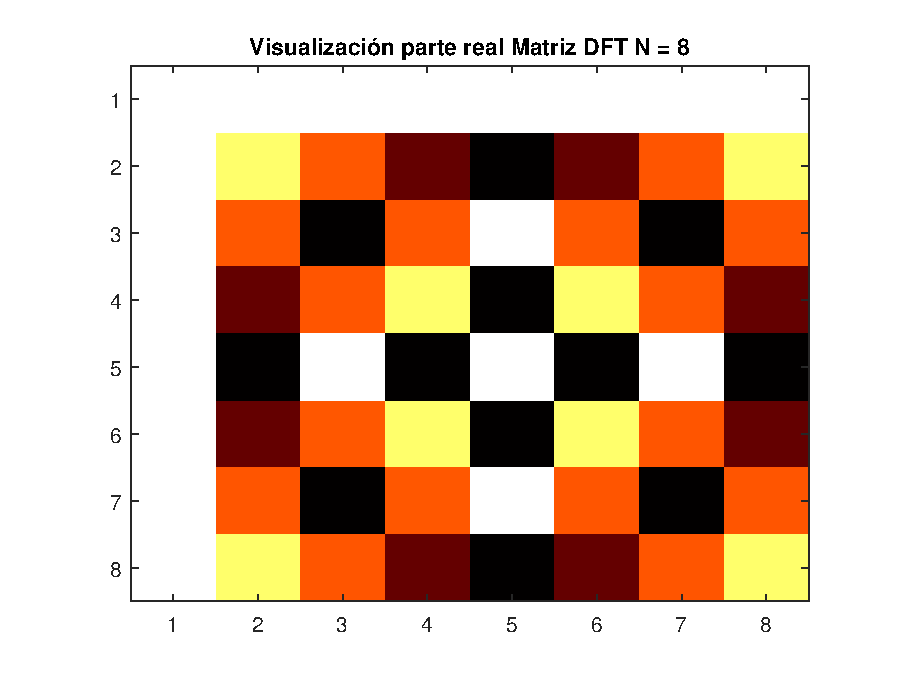
\includegraphics[width = .7\linewidth]{Figuras/P5_2_1.eps}
        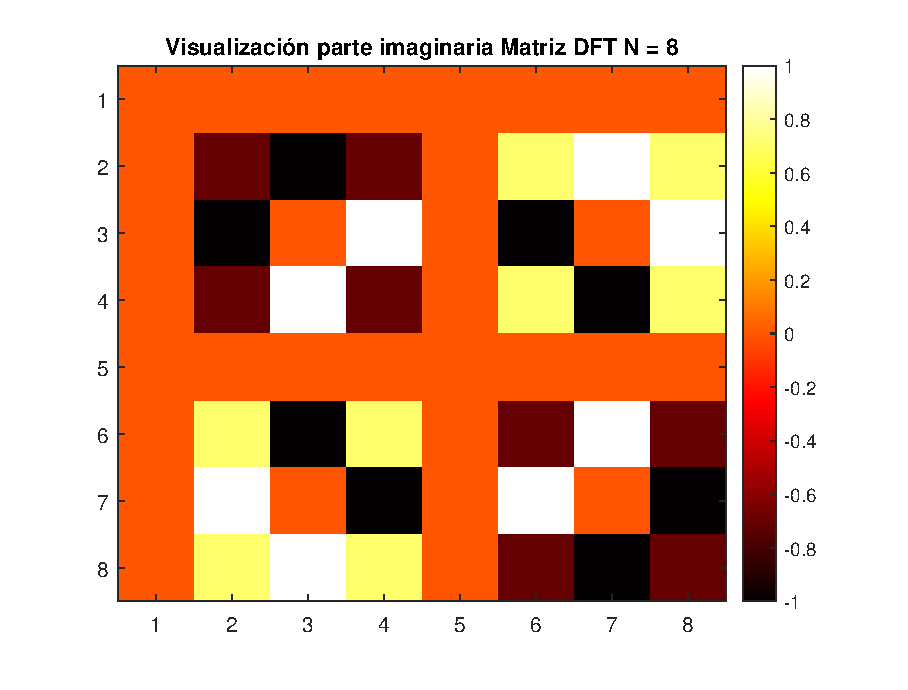
\includegraphics[width = .7\linewidth]{Figuras/P5_2_2.eps}
        \caption{Visualización parte real e imaginaria de matriz DFT de 8 puntos.}
        \label{fig:p5_2n8}
    \end{figure}
    
    Las matrices de la DFT de 64 puntos se muestran en la figura \ref{fig:p5_2n64}.
    
    No se aprecian diferencias en las simetrías apreciadas en la parte real e imaginaria con respecto a la matriz de 8 puntos.
    
    \begin{figure} [H]
        \centering
        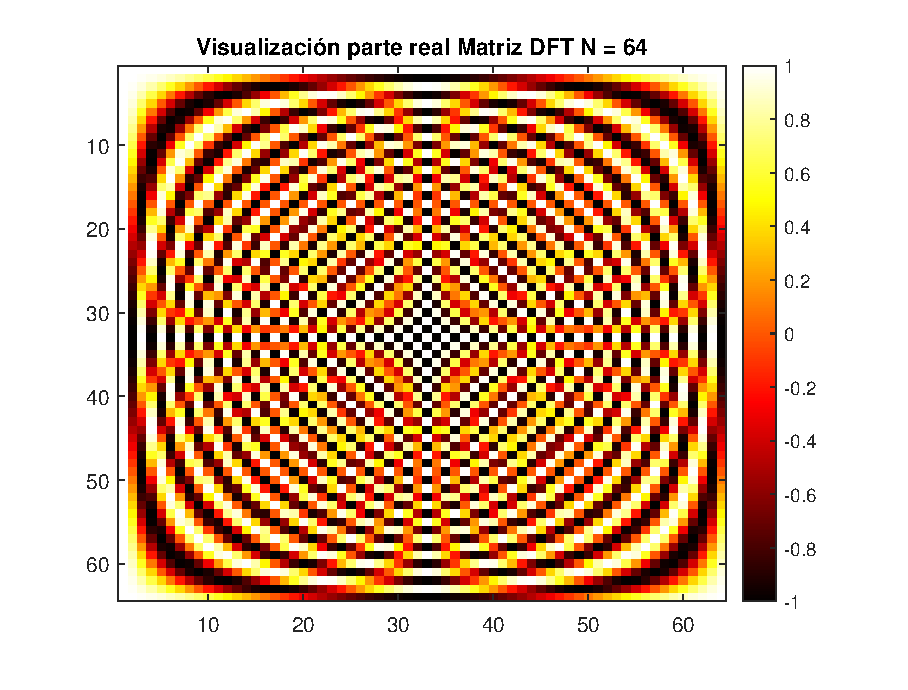
\includegraphics[width = .7\linewidth]{Figuras/P5_2_3.eps}
        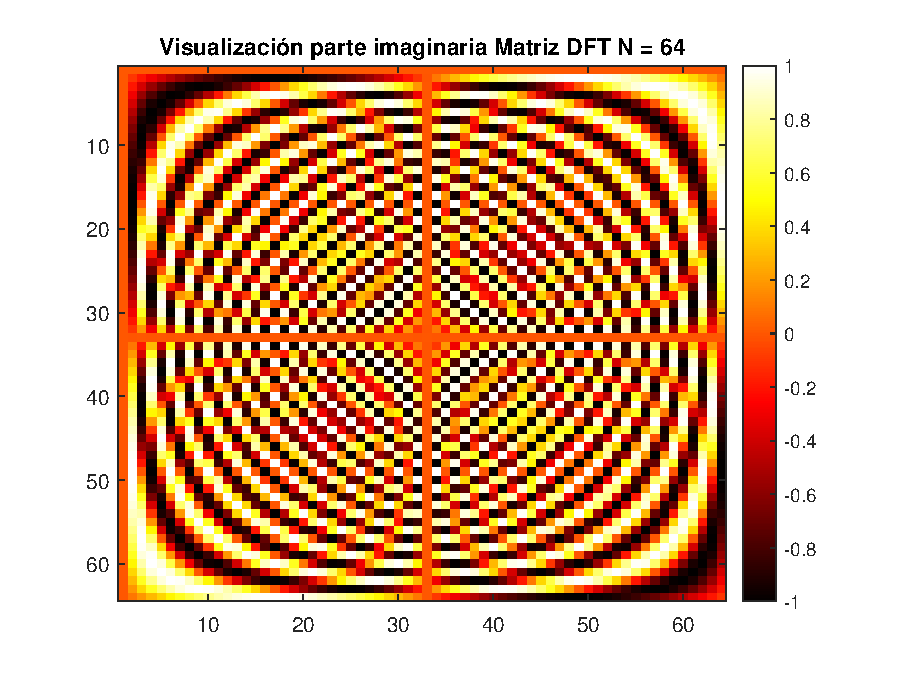
\includegraphics[width = .7\linewidth]{Figuras/P5_2_4.eps}
        \caption{Visualización parte real e imaginaria de matriz DFT de 64 puntos.}
        \label{fig:p5_2n64}
    \end{figure}
    
    
    %5.3
    \item Para probar la implementación de la función \texttt{DFTmatrix(x)}, se procede de la misma forma que al probar la implementación de la función \texttt{DFTsum(x)} del inciso anterior. Se usan las mismas señales $x1,x_2,x_3$ y $x_4$ también con 8 muestras para cada una de ellas. Se grafica la para cada señal el resultado entregado por la función implementada así como el resultado que se obtiene haciendo uso del comando \textit{fft} de MATLAB. Las gráficas mencionadas se muestran en la figura  \ref{DFTmatrix}
    
    
    \begin{figure}[H]
        \centering
        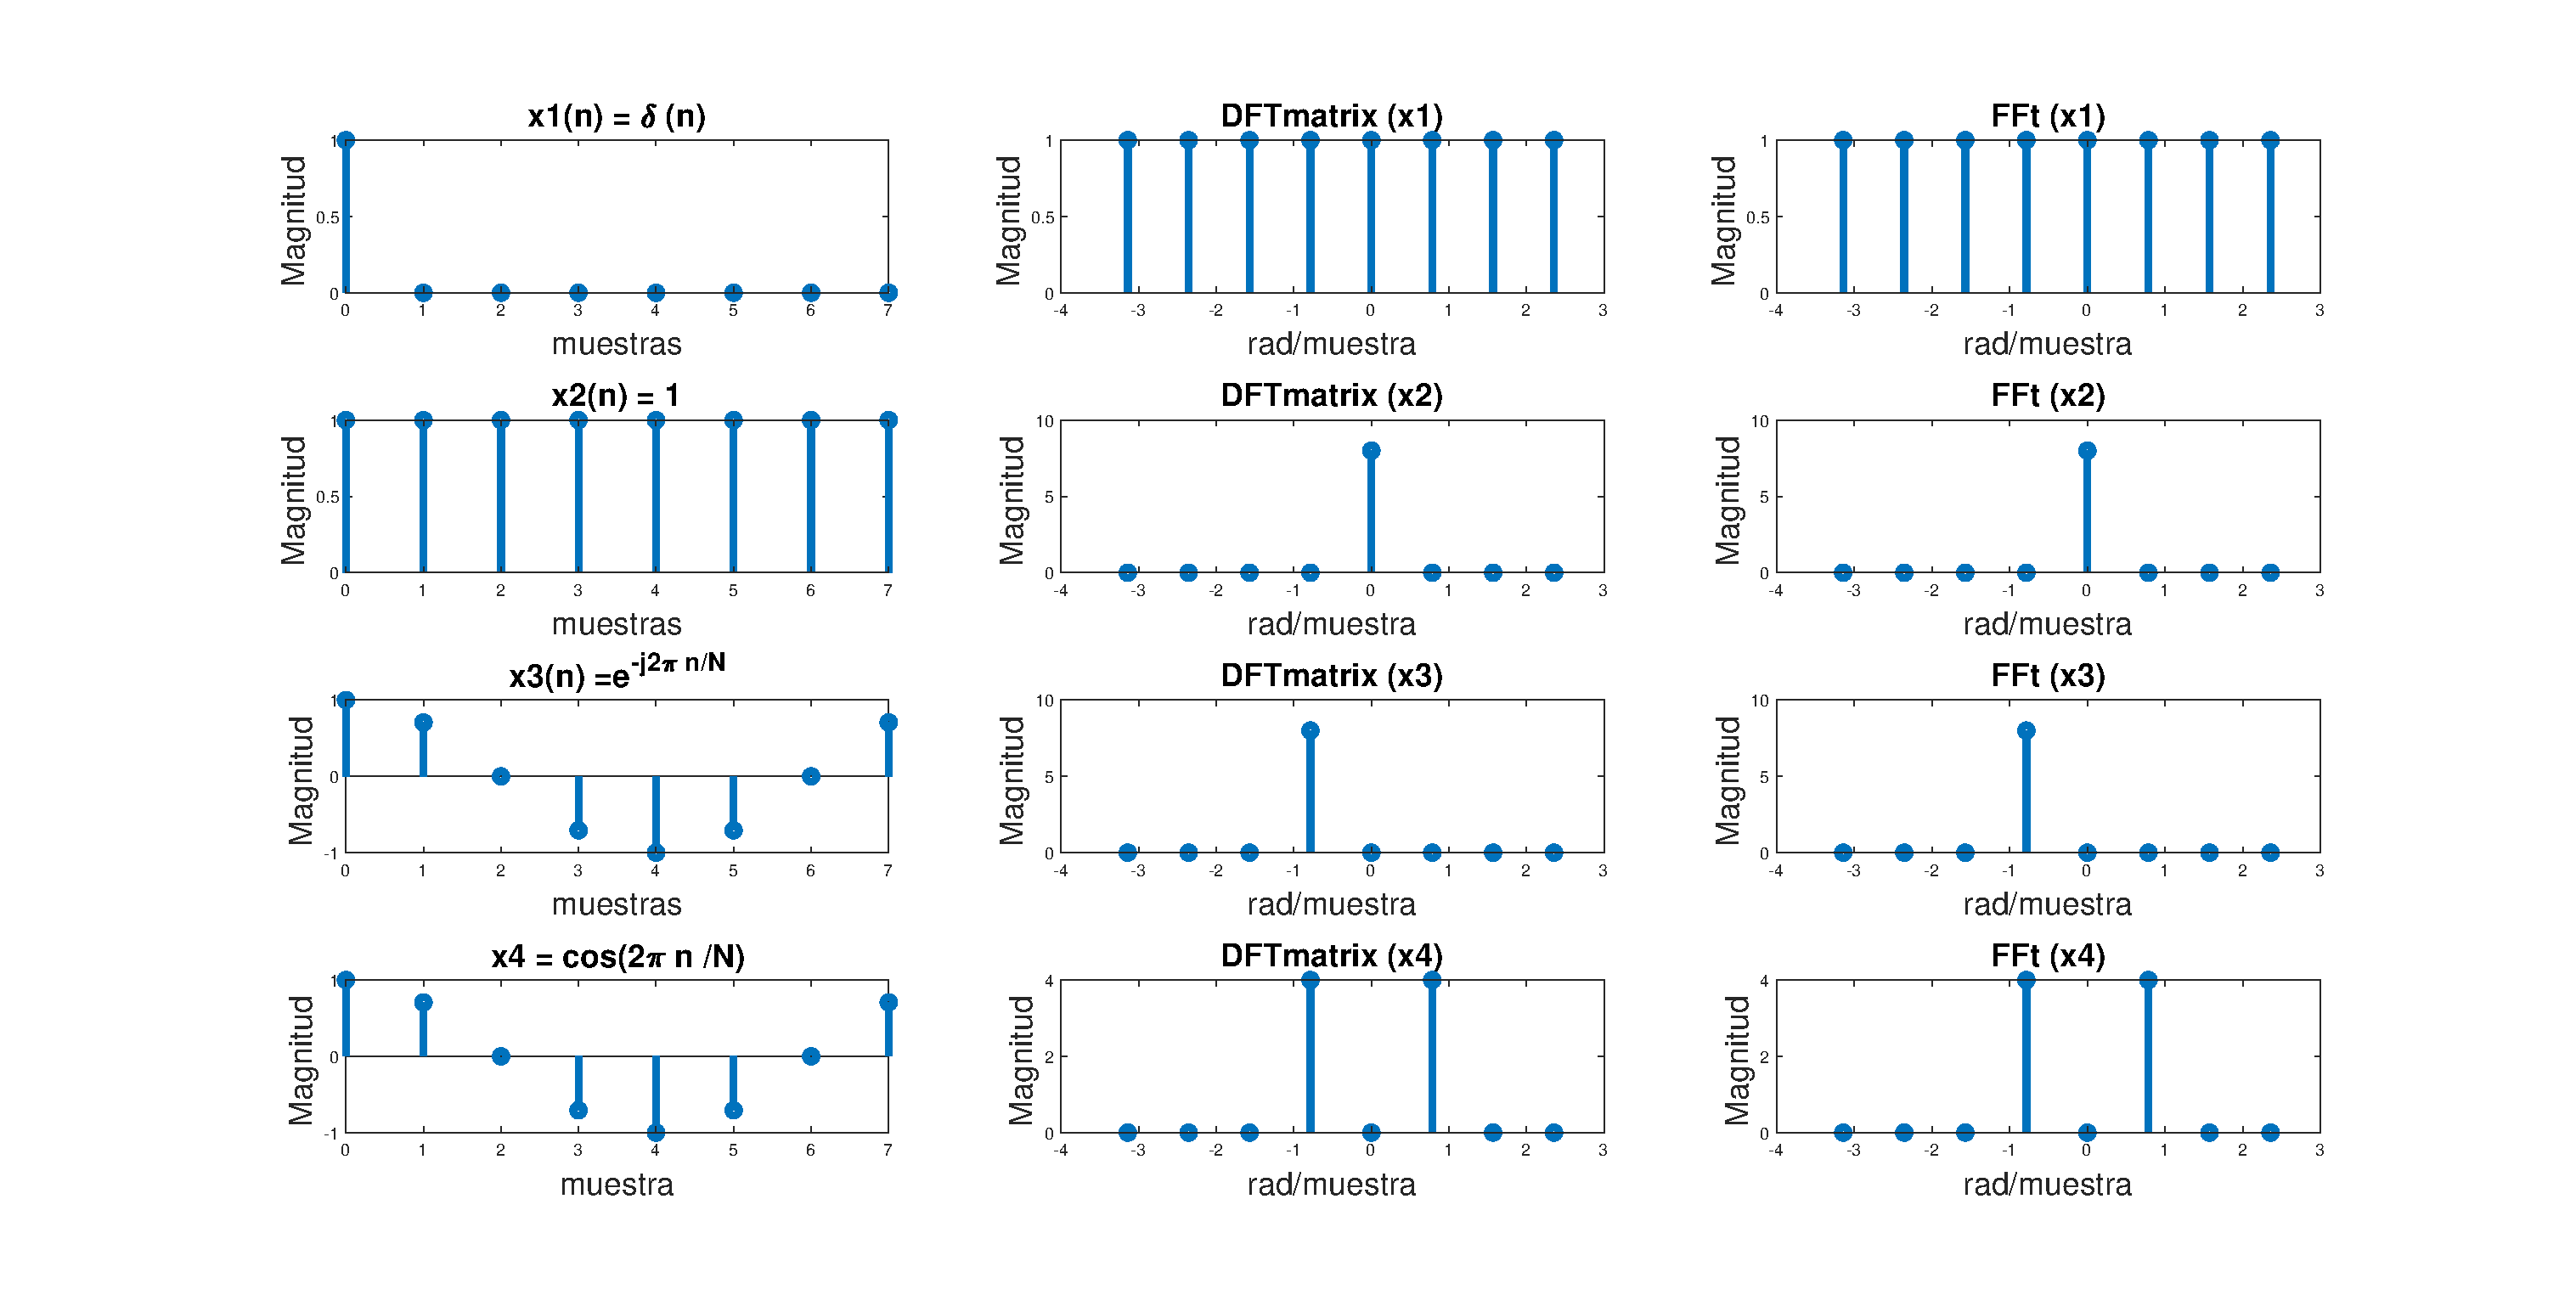
\includegraphics[scale = 0.3]{Figuras/p4_1-DFTmatrix.eps}
        \caption{Señales $x_1$, $x_2$, $x_3$ y $x_4$ generadas junto a sus respectivas DFT obtenida con la función implementada y FFT obtenida con comandos en MATLAB}
        \label{DFTmatrix}
    \end{figure}


Como se puede apreciar en las gráficas, al igual que en el caso anterior con la función \texttt{DFTsum(x)}, esta vez para la función \texttt{DFTmatrix(x)} se obtienen resultados cualitativamente idénticos a los que se obtienen haciendo uso del comando \textit{fft} de MATLAB. Cabe mencionar que nuevamente para el caso de la señal $x_3$ se ha graficado unicamente la parte real correspondiente.

A continuación se presenta una tabla con los errores cuadráticos medios asociados a ambas funciones implementadas que homologan el comportamiento del comando \textit{fft} de MATLAB.


  
 
 \begin{table}[H]
        \centering
        \begin{tabular}{|c|c|c|}
        \hline
         Señal    & MSE DFTsum $v/s$ fft & MSE DFTmatrix $v/s$ fft  \\
         \hline
         $x_1(n) = \delta (n)$   & $0$ & $0$ \\
         \hline
          $x_2(n) = 1$   &   $1.2195\cdot 10^{-30}$  & $3.8323\cdot 10^{-30}$\\
         \hline
            $ x_3(n) =e^{-j2 \pi n /N}$ &   $7.1631\cdot 10^{-31} $ & $3.8254\cdot 10^{-30}$  \\
         \hline
        
         $ x_4(n) = cos(2\pi n /N)$  &    $3.1880\cdot 10{-31}  $ & $5.9170\cdot 10^{-31}$\\
         \hline


        \end{tabular}
        \caption{Cuadro resumen para el error cuadrático medio entre el resultado de las funciones \texttt{DFTsum} y  \texttt{DFTmatrix} con respecto al resultado entregado por el comando \texttt{fft} de MATLAB para cada señal de prueba.}
        \label{MSE}
    \end{table}
    
    Todos los errores encontrados son despreciables ya que su orden de magnitud no es significativo respecto a las magnitudes con las que se trabaja en el contexto actual.
    

    %5.4
    \item Se utiliza el comando \texttt{timeit} de MATLAB para medir el tiempo de procesamiento de los métodos $fft, DFTsum$ y $dftmtx$, considerando $N = (100:100:5000)$ puntos.   
    
    Se grafica el tiempo de procesamiento para los valores de $N$, donde se escoge escala logarítmica para fines comparativo. El gráfico se muestra en la figura \ref{fig:p5_4cmp}. 
    
    \begin{figure}[H]
        \centering
        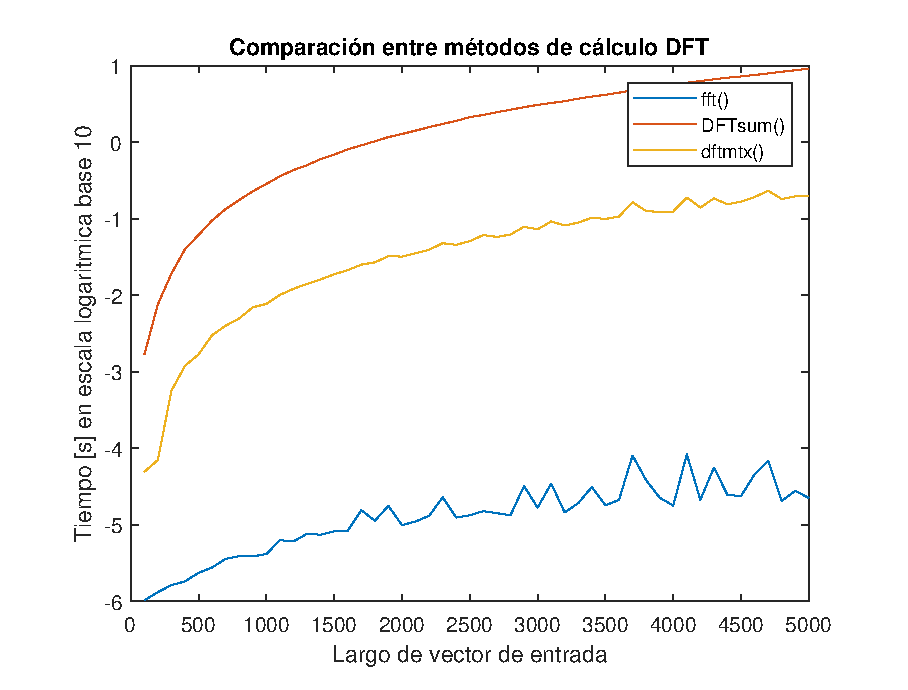
\includegraphics[width = .8\linewidth]{Figuras/p5_4cmp.eps}
        \caption{Tiempo de procesamiento para funciones $fft, DFTsum$ y $dftmtx$, considerando $N = (100:100:5000)$ puntos.}
        \label{fig:p5_4cmp}
    \end{figure}
    
    Con respecto al tiempo de procesamiento se concluye que:
    \begin{itemize}
        \item Para los largos probados de entrada, la $fft$ resulta más rápida que el método $dftmtx$ y este a su vez que el $DFTmtx$.
        \item La razón del tiempo de procesamiento entre $DFTsum$ y $fft$ es de aproximadamente $10^{-6}$, a partir de largos de 1000 muestras. Antes de las 1000 muestras la razón va en ascenso
        \item La razón del tiempo de procesamiento entre $DFTsum$ y $fft$ es de aproximadamente $10^{-4}$, a partir de largos de 1000 muestras.  Antes de las 1000 muestras la razón va en ascenso.
        \item La La razón del tiempo de procesamiento entre $DFTsum$ y $dftmtx$ es aproximadamente $10^{-2}$, para todos los largos de datos probados.
    \end{itemize}
    
    Con respecto a la memoria utilizada, claramente el método $dftmtx$ es el que ocupa más debido a que gerena la matriz de transformación que termina siendo de $N\times N$
    
    

    


    
    \end{enumerate} 
    


